\chapter{Grundlagen}
\label{chap:grundlagen}

In diesem Abschnitt meiner Arbeit, möchte ich zu erst die nötigen Grundlagen behandeln, um ein Basiswissen für die folgenden Kapitel sicherzustellen.
Da sich die Arbeit hauptsächlich um den Bildmerkmal Algorithmus \textbf{Histogram of Oriented Gradients} Algorithmus dreht, fange ich mit diesem an.
\section{Histogram of Oriented Gradients}
\label{sec:grundlagenhog}
Wie gerade erwähnt ist der \textbf{HOG} ein Bildmerkmal Algorithmus, der sich gegen bekannte Algorithmen (z.B. SIFT) bestens schlägt und dabei  effizienter arbeitet. Entwickelt und vorgestellt wurde der Algorithmus von Navneet Dalal und Bill Triggs im Paper $Histograms~of ~oriented~Gradients~for~Human~Detection$ \cite{dalal:inria-00548512} veröffentlicht.
Grundlegend funktioniert der Algorithmus durch das Beschreiben von Verläufen. Diese Informationen werden in ein geeignetes Format gebracht um anschließend das betrachtete Bild zu klassifizieren. Wie in der ursprünglichen Arbeit, wird in dieser Arbeit erkannt ob ein Mensch in  einem Bild vorhanden ist.
Den gesamten Ablauf kann man in Abbildung 2.1 sehen. Da einige Schritte für das Verständnis nicht erforderlich sind, werde ich nur einen Teil dieser erklären.

\begin{figure}[htbp]\centering 
	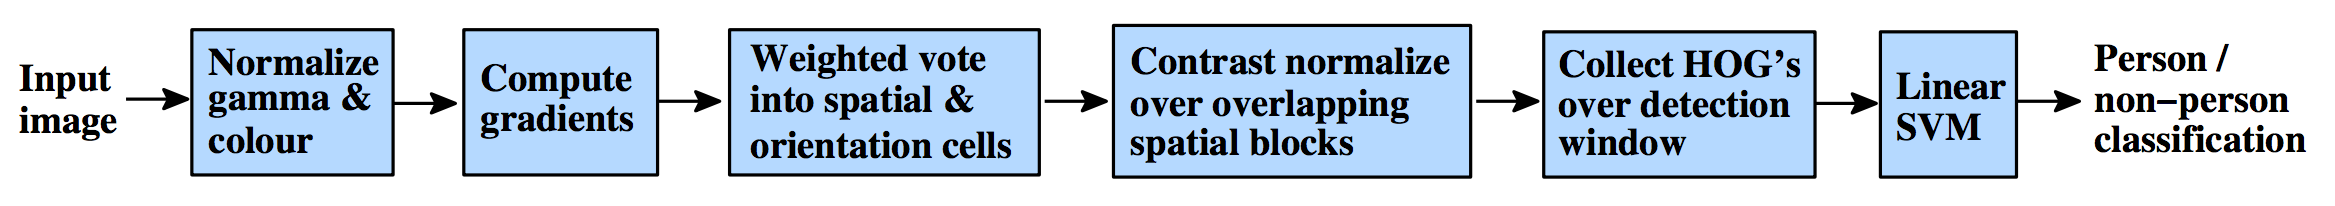
\includegraphics[width=1\linewidth]{pics/feature extraction chain.png} 
	\caption{Ablauf der Klassifizierung von Bildmerkmalen
	\cite{dalal:inria-00548512}}\label{fig:grundlagen_feature_extraction_chain}\end{figure}

Die wichtigsten Bestandteile werde ich im Folgenden erklären.

\subsection{Gradienten-Vektoren}

Wie der Name zu erkennen gibt, betrachtet der \textbf{HOG}-Algorithmus die Gradienten eines Bildes. Beschrieben werden Gradienten durch Vektoren:

$$
\vec{g}=\begin{pmatrix}
	g_x \\
	g_y
\end{pmatrix}
$$

Um die Elemente $g_x$ und $g_y$ zu berechnen, gibt es einige mögliche Filter. Laut $Dalal$ und $Triggs$ \cite[S.5]{dalal:inria-00548512} funktioniert der simple Filter

$$
\vec{x}=\begin{pmatrix}
	-1 & 0 & 1
\end{pmatrix}
$$
bzw.
$$
\vec{y}=\begin{pmatrix}
	-1 \\
	0 \\
	1
\end{pmatrix}
$$
am besten.
Diese Filter werden auf jeden Bildpunkt im Bild angewandt. Somit ergibt sich die Berechnung von $g_x$ und $g_y$ zu:
\begin{equation*}
	g_{x_k}=-x_{k-1}+x_{k+1} \\
	g_{y_k}=-y_{k-1}+y_{k+1}
\end{equation*}

Dabei ist $x_k$ der betrachtete horizontale Bildpunkt und $y_k$ ist der betrachtete vertikale Bildpunkt.
Jedoch aufgepasst, man muss beachten, dass bei einem Farbbild $g_x$ und $g_y$ für jeden Farbkanal berechnet werden müssen. Zusätzlich verhält sich die Berechnung am Rand des Bildes etwas anders.
Wie in der Abbildung ... dargestellt, wird der Wert des Bildpunktes am Rand für die Berechnung einfach wiederholt.

\begin{table}[h!]
\centering
\caption{ANSTATT TABELL, ZEICHNEN!!!Randverhalten!!!}
\label{fig:randverhalten}
\begin{tabular}{c|
>{\columncolor[HTML]{FFFE65}}c |
>{\columncolor[HTML]{FFFE65}}c |
>{\columncolor[HTML]{FFFE65}}c |c}
\cline{2-4}
                                                  & \cellcolor[HTML]{C0C0C0}56 & \cellcolor[HTML]{C0C0C0}... & \cellcolor[HTML]{C0C0C0}98 &                                                  \\ \hline
\multicolumn{1}{|c|}{\cellcolor[HTML]{C0C0C0}56}  & 56                         & ...                         & 98                         & \multicolumn{1}{c|}{\cellcolor[HTML]{C0C0C0}98}  \\ \hline
\multicolumn{1}{|c|}{\cellcolor[HTML]{C0C0C0}...} & ...                        & ...                         & ...                        & \multicolumn{1}{c|}{\cellcolor[HTML]{C0C0C0}...} \\ \hline
\multicolumn{1}{|c|}{\cellcolor[HTML]{C0C0C0}67}  & 67                         & ...                         & 34                         & \multicolumn{1}{c|}{\cellcolor[HTML]{C0C0C0}34}  \\ \hline
                                                  & \cellcolor[HTML]{C0C0C0}67 & \cellcolor[HTML]{C0C0C0}... & \cellcolor[HTML]{C0C0C0}34 &                                                  \\ \cline{2-4}
\end{tabular}
\end{table}

Um nun Histogramme zu erstellen benötigt man für den HOG-Algorithmus zwei Werte. Einmal die Magnitude des Gradienten und dessen Orientierung.
Die Magnitude wird nach dem Satz von Pythagoras durch:
$$ \lvert G \rvert=\sqrt{g_{x_k}^{2}+g_{y_k}^{2}} $$
berechnet und die Orientierung durch:
$$ \theta=\arctan\frac{g_{x_k}}{g_{y_k}} $$.
Die Histogramme entstehen nun durch gewichtetes $binning$ (die Gruppierung zu Intervalle). 

\section{Support Vector Machine}
\label{sec:grundlagensvm}

\section{Tensilica Xtensa LX5}
\label{sec:grundlagenlx5}

\section{Tensilica Instruction Extension}
\label{sec:grundlagentie}

\section{Assembler}
\label{sec:grundlagenassembler}				